\chapter{Wilson loops}\label{ch:WilsonLoops}


A Wilson loop is a gauge-invariant observable, 
defined as the expectation value of the character of the representation $\mathcal{R}$ of the gauge group 
($U(N)$ in our case):
\begin{equation}
  W_{\mathcal{R}}(C) =  \left\langle \text{tr}_{\mathcal{R}} U \right\rangle, \quad U \in U(N)
  %\dfrac{1}{\text{dim}\, \mathcal{R}}
\end{equation}
where $U$ is a path-ordered exponential of the gauge connection $A_\mu$, 
transported along an arbitrary curve $C$ parametrized by $s$:
\begin{equation}
 U = \mathop{\mathrm{P}}\exp 
    \left[ 
	i \int_C ds\,	
	  \dot{x}^\mu A_\mu
    \right],
\end{equation}
where the dot denotes derivative respect $s$.

Physically, the Wilson loop operator measures the phase associated with moving a probe particle with charge
$\mathcal{R}$ around a curve $C$ in spacetime.
In particular, the long rectangular Wilson loop in the fundamental representation, the path shown in the figure \ref{fig:WLrectangle},
determines the static quark and antiquark potential:
\begin{equation}
 V_{q\bar{q}} (L) = -\dfrac{1}{T} \lim_{T\rightarrow\infty} \log W_1(C).
\end{equation}
In confined theories such as QCD, the potential is linear,
% $V_{q\bar{q}} (L) \propto L$, 
which is referred as the \emph{area law} in terms of the Wilson loop,
$\log W \propto L\times T$,
while in the deconfined phase, the Wilson loop follows the \emph{perimeter law},  $\log W \propto L$.


\begin{figure}[t]
\begin{center}
 \centerline{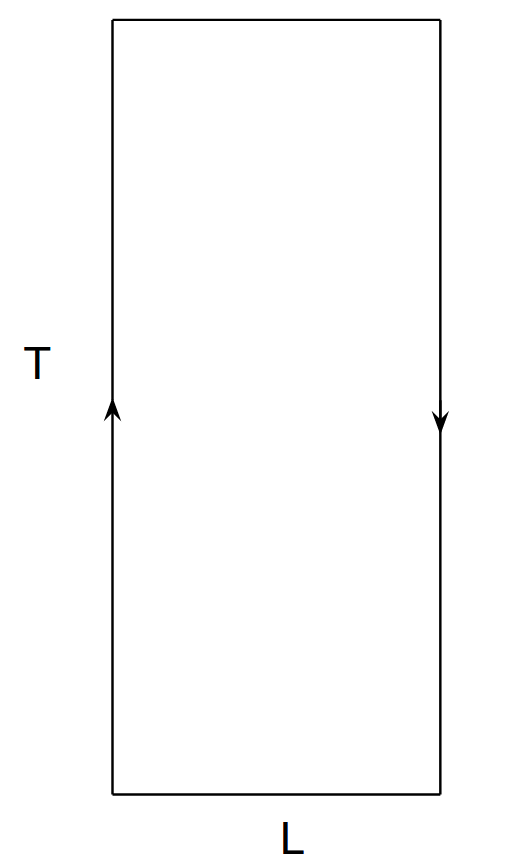
\includegraphics[width=4cm]{Images/WLrectangle.png}}
\end{center}
\caption{\label{fig:WLrectangle} Trajectory of a probe quark and antiquark separated by distance $L$, and travel $T$ distance in time. }
\end{figure}


We are interested in a supersymmetric extension of the Wilson loop,
such that it is computable through localization, see conditions \eqref{loc:susyCondition}.
We will study the so-called Maldacena-Wilson loop \cite{Maldacena:1998im},
where we add a coupling to the scalars of the vector multiplet:
\begin{equation} \label{maldacenaWL}
 U = \mathop{\mathrm{P}}\exp 
    \left[ 
	\int_C ds\,
	\left(
	  i\dot{x}^\mu A_\mu +|\dot{x}|n^I\Phi_I 
	\right)
    \right], \quad I=0,9.
\end{equation}
% where $n^I$ are components of the unit vector that parametrizes $S^5$.
Let us start by reviewing some known results in $\mathcal{N}=4$ SYM and then generalize them to $\mathcal{N}=2^*$.



\section{Wilson loops in $\mathcal{N}=4$ SYM}

The simplest Wilson loop is an infinite straight line. 
It is a half-BPS object, meaning it commutes with half of the 32 supercharges of $\mathcal{N}=4$ SYM.
This fact protects the Wilson line from quantum corrections and its value is simply one:
\begin{equation}
 \braket{W_\text{line}} = 1.
\end{equation}


By conformal transformation, the Wilson line can be mapped to a circular Wilson loop.
The result, however, is not the same. 
This is often referred to as a conformal anomaly, 
and it is due to the fact that large conformal transformations such as inversion are not symmetries in the flat space
(infinity is not a point of $\mathbb{R}^d$). 
On the sphere, these are symmetries, hence there is no distinction between a circle and a line, and the
expectation value of either is the same as for a circle on $\mathbb{R}^4$ \cite{Drukker:2000rr}.
The circular Wilson loop, which is also half-BPS, is exactly computable using the localized partition function for the theory on $S^4$,
where the path is the equator of sphere, see figure \ref{fig:equatorWL}.

\begin{figure}[t]
\begin{center}
 \centerline{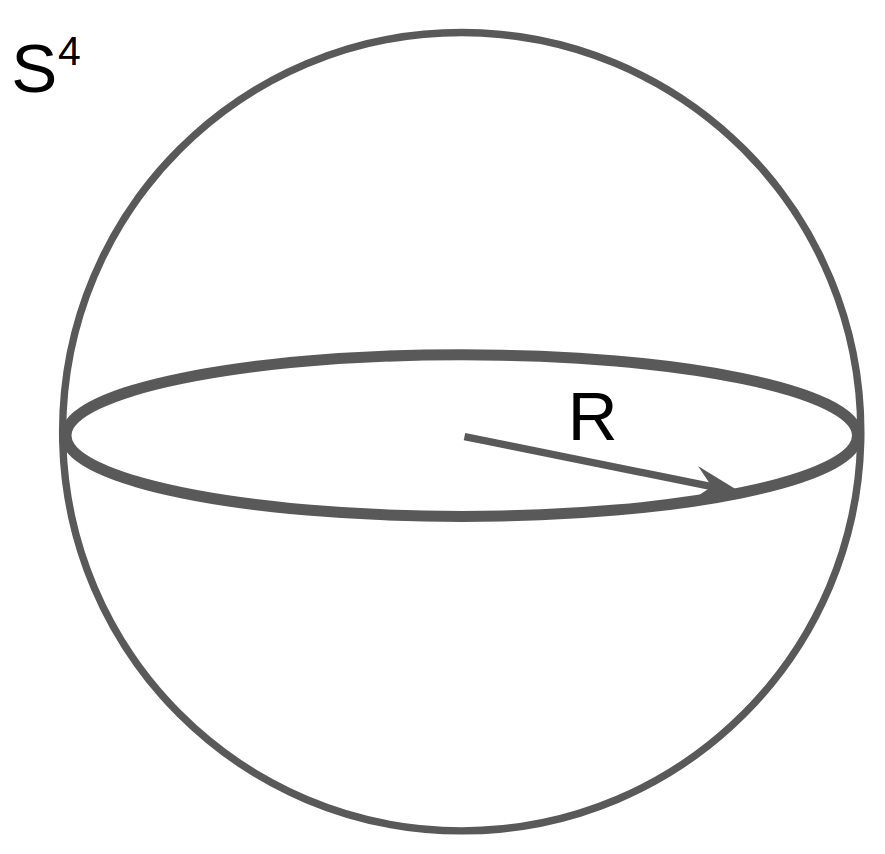
\includegraphics[width=4cm]{Images/equatorWL.png}}
\end{center}
\caption{\label{fig:equatorWL} The contour of the circular Wilson loop we study is the equator of the hypersphere the theory is defined on.}
\end{figure}


\subsection{Fundamental representation}
The circular Wilson loop in the fundamental representation is mapped to a matrix model expectation value:
\begin{equation}\label{eq:W1mm}
 W_1 = \left< \dfrac{1}{N}\sum_{i=1}^N e^{2\pi a_i} \right>_\text{matrix model},
%  \overset{N \gg 1}{\approx} \int_{-\mu}^{\mu} dx\, \rho(x) \,e^{2\pi x}
\end{equation}
which can be solved exactly for GUE \cite{Drukker:2000rr}:
\begin{equation}
 W_1 = \dfrac{1}{N} L_{N-1}^1 (-\lambda/(4N)) e^\frac{\lambda}{8N},
\end{equation}
where $L$ is the generalized Laguerre polynomial:
\begin{equation}
 L_n^m(x)=\dfrac{x^{-m}  e^x}{n!}\,  \dfrac{d^n}{dx^n}(e^{-x} x^{n+m}).
\end{equation}

In the large $N$ limit and fixed 't Hooft coupling, 
\eqref{eq:W1mm} can be written as:
\begin{eqnarray}
 W_1 &=& \int_{-\mu}^{\mu} dx\, \rho(x) \,e^{2\pi x} \label{eq:W1continuous} \\
     &=& \dfrac{2}{\sqrt{\lambda}} I_1 (\sqrt{\lambda}), \quad (N\rightarrow \infty \quad \text{and} \quad \lambda \text{ - fixed})
\end{eqnarray}
where for the last equality, we used the semicircle distribution \eqref{semicircle},
since the Wilson loop insertion to the partition function is subleading in $N$.
$I_1(x)$ is the modified Bessel function:
\begin{equation}
 I_1(x) = \sum_{n=0}^\infty  \dfrac{1}{n! (n+1)!} \left(\dfrac{x}{2}\right)^{2n+1}.
\end{equation}


Historically, the large-$N$ result was initially obtained by Erickson-Semenoff-Zarembo \cite{Erickson:2000af},
by summing over rainbow diagrams in perturbation theory, and they conjectured the Gaussian matrix model structure for $\mathcal{N}=4$ SYM.
Eventually Pestun's work in localization \cite{Pestun:2007rz} proved it.



In the 't Hooft limit, which is the holographic regime, 
\begin{equation}\label{W1holographic}
 W_1 = \sqrt{\frac{2}{\pi}} \lambda^{-3/4} e^{\sqrt{\lambda}}, 
 \quad (N\rightarrow \infty \quad \text{and} \quad \lambda \rightarrow \infty).
\end{equation}
% which matches with the minimal surface of the worldsheet with boundary $C$, drawn by the classical string on the supergravity background.
% We will discuss more on the holographic dual in another chapter.
% The subleading order term comes from the measure of the path integral, and so far, 
% it is still an open problem that many attempted to solve (cite Papers). 

% The equatorial Wilson loops can be generalized to latitude Wilson loops, 
% though the latter are less supersymmetric, and belongs to the family of 1/4 BPS.
% Their exact result can be obtained by just rescaling the 1/2 BPS, by 
% $\lambda \rightarrow \lambda \cos^2\theta_0$, 
% where the angle $\theta_0$ is the polar angle of the latitude.


\subsection{Higher rank representations}

Exact results for arbitrary representation of $U(N)$ can also be obtained \cite{Fiol:2013hna}.
These are very generic, though, 
but the generating function of $k$-antisymmetric representation 
\begin{equation}\label{eq:generatingFunctionAk}
 \braket{G_{A_k}(t)}=\sum_{k=0}^{N} t^k \, W_{A_k}
\end{equation}
has a nice compact form:
\begin{equation}
 \braket{G_{A_k}(t)}=\text{det}\left(t \delta_{ij}+ L_{i-1}^{j-i}(-\lambda/(4N)) e^{\frac{\lambda}{8N}}\right).
\end{equation}

We study the 't Hooft limit
for the symmetric (+) and the antisymmetric (-) representations. 
The generating functions\footnote{
Here, unlike in \eqref{eq:generatingFunctionAk}, 
we use the expansion parameter $e^{-\nu}$ instead of $t$.}
for the character of these representations are explicitly known:
\begin{equation}
 G_k^{\pm}(\nu) = \prod_{i=1}^N (1\mp e^{a_i - \nu})^{\mp}.
\end{equation}
Notice that these are also the Bose (+) and Fermi (-) distributions, in terms of the eigenvalues $a_i$.

The standard procedure is to derive the character by inverting the generating function using Cauchy's integral formula:
\begin{equation}\label{eq:characterIntegral}
 \chi_k^\pm \equiv \text{tr}_\pm \,U = \int_{C-i\pi}^{C+i\pi} \dfrac{d\nu}{2\pi i} \, e^{\nu k} G_k^\pm(\nu),
\end{equation}
where $C>a_i, \forall i$, for the symmetric case, and $C$ is arbitrary for the antisymmetric case.


All we need to do now is to compute the expectation value of the above integral. 
We can still employ the semicircle distribution \eqref{semicircle}, 
and we further take the large representation limit $k \sim N$,
which allows us to use the saddle-point method in \eqref{eq:characterIntegral}, \cite{Hartnoll:2006is}.
The saddle-point equation to solve for $\nu_*$ is
\begin{equation}\label{eq:saddlePointDensity}
 \dfrac{k}{N} = \int_{-\mu}^\mu dx \, \dfrac{\rho(x)}{e^{L(\nu_*-x)}\mp 1}, 
 \quad (N\rightarrow \infty \quad \text{and} \quad \frac{k}{N} \text{ - fixed}),
\end{equation}
which is analogous to the particle density equation in a Bose/Fermi system.

The final leading solutions for the antisymmetric representation is
\begin{equation}\label{solW-}
 \log W_{k}^-= N \frac{2\sqrt{\lambda }}{3\pi}\,\sin^3\theta, 
\end{equation}
where $\cos \theta\equiv \nu_*/\mu$ satisfies the transcendental equation
\begin{equation}\label{eqThetaAntisym}
 \theta -\frac{1}{2}\,\sin 2\theta =\pi \frac{k}{N},
\end{equation}
resulting from \eqref{eq:saddlePointDensity}
after the step-function approximation of the Fermi distribution.

For the symmetric representation, however, 
there is no saddle-point solution for \eqref{eq:saddlePointDensity}. 
This is the same phenomenon as the Bose-Einstein condensation.
It is possible to analytically continue the solution to the second Riemann sheet, though, 
as done in \cite{Hartnoll:2006is},
and the final result is:
\begin{equation}\label{solW+}
 \log W_{k}^+ = 2 N  f\left(\kappa\right),  
 \quad  \kappa \equiv \frac{\sqrt{\lambda }\,k}{4 \,N}
\end{equation}
where 
\begin{equation}\label{eqfSym}
 f(x) = x\sqrt{1+x^2}+\mathop{\mathrm{arcsinh}}x.
\end{equation}

The drawback of the analytic continuation was that computing large-$N$ corrections became less clear, as attempted in \cite{Faraggi:2014tna}.
In Paper II and Paper IV, we used a more systematic approach.
Paper IV focused exclusively on the symmetric Wilson loop in $\mathcal{N}=4$ SYM, 
where subleading corrections in $N$ were computed.
This result is consistent with the expansion of the known exact result for the multiply wrapped fundamental Wilson loop \cite{Kawamoto:2008gp},
which helped to clarify the apparent mismatch observed in \cite{Faraggi:2014tna},
and agrees with the analysis by \cite{Yamaguchi:2007ps} that symmetric representations and the multiply-wound fundamental ones 
differ by exponentially-suppressed terms in strong coupling.
Paper IV also derived the strong-coupling corrections, 
in response to the strong-coupling expansion done for the antisymmetric case in \cite{Horikoshi:2016hds},
where the Sommerfeld expansion of the Fermi distribution was used.
%k-fundamental obtained by relplacing $\lambda \rightarrow k^2 \lambda$.




\section{Wilson loops in $\mathcal{N}=2^*$ SYM}

The story can be extended to $\mathcal{N}=2^*$ SYM on $S^4$.
Here we have an extra parameter: the scale $MR$.
We will take the decompactification limit $MR \rightarrow \infty$, where interesting phase transitions were seen, 
and also, the dual theory is fully known on $\mathbb{R}^4$ \cite{Pilch:2000ue}.
% (the dual on $S^4$ is partially known, \cite{Bobev:2013cja}).

% We work with the equatorial circular Wilson loop and reasonably assume that results in the decompactification limit is universal for any large contour.


\subsection{Fundamental representation}

Since the fundamental Wilson loop is basically an exponentially-weighted integral \eqref{eq:W1continuous},
its value in the strong coupling limit is determined by the largest eigenvalue $\mu$
(recall $\mu\sim\sqrt{\lambda}$, see \eqref{semicircleN=2*}). 
Thus, we do not expect its strong coupling corrections to probe the cusps region.
In Paper I, we computed the subleading correction to the endpoint $\mu$,
which lead to the same correction to the Wilson loop (in terms of the perimeter $l=2\pi R$):
\begin{equation}\label{WLFundN2}
 \log W_1= P(\lambda) Ml, \quad P(\lambda) = \frac{\sqrt{\lambda}}{2 \pi} -\frac{1}{2} + \mathcal{O}\left(\dfrac{1}{\sqrt{\lambda}}\right), 
 \quad (MR\rightarrow \infty).
\end{equation}
The leading order term is the same as its homologous case in $\mathcal{N}=4$, only rescaled by $MR$ \cite{Buchel:2013id},
as a direct consequence of the semicircle behavior of the bulk distribution \eqref{semicircleN=2*}.
As a consistent check, when $M\rightarrow 0$, the Wilson loop goes to 1, as expected for the $\mathcal{N}=4$ case.
Moreover, we clearly see the perimeter law here since the theory is not confining neither conformal.



\subsection{Symmetric and antisymmetric representations}
In Paper II, result for symmetric and antisymmetric representations were computed,
up to the next-to-leading order in the strong coupling expansion.
The decompactified results at the leading order in $N$ are also the same as the ones in the $\mathcal{N}=4$ case,
but rescaled differently:
\begin{eqnarray}
 \log W_{k}^- &=& N M R\frac{2\sqrt{\lambda }}{3\pi}\,\sin^3\theta,\\
 \log W_{k}^+ &=& 2 N (MR)^2 f\left(\frac{\kappa}{M R}\right),
\end{eqnarray}
where $\theta$ and  $f$ satisfy the same equation as in \eqref{eqThetaAntisym} and \eqref{eqfSym}, respectively.

Now, the interesting part lays in the subleading terms. 
Unlike the fundamental representation, the higher rank representations do probe the endpoint distribution of the eigenvalues, 
which has periodic cusps with period $MR$, see figure \ref{fig:phaseDiagram}.
The results are:
\begin{equation}\label{WantisymPW}
 \delta \log W_{k}^- = -\dfrac{2\pi^2}{3} \dfrac{N M R}{\lambda^{3/4}}
\begin{cases}
 4\tilde{f}^3 & {\rm }0<\tilde{f}\leq 1
\\
 \tilde{f}^3+6\tilde{f}-\frac{3}{\tilde{f}} & {\rm } 1<\tilde{f}\leq 1+\sqrt{2}
 \\
 \vdots &
\end{cases}, \quad 
\tilde{f} = \dfrac{\lambda^{3/4} k }{ 4\sqrt{\pi} N}
\end{equation}
and
\begin{equation}\label{WsymPW}
 \delta \log W_{k}^+ = \dfrac{2^5\pi^{3/2}}{5}\dfrac{N (M R)^2}{\lambda^{3/4}} \left(v^{5/2}+\Theta(v-1)\left(v+\dfrac{2}{3}\right)(v-1)^{3/2}\right), 
\end{equation}
where $\Theta(x)$ is the Heaviside function and $v$ is written in terms of the scaling parameter $\tilde{f}$ as
\begin{equation}
  \dfrac{3}{2}\tilde{f} = v^{3/2}-\Theta(v-1)(v-1)^{3/2}, \quad \tilde{f} = \dfrac{\lambda^{3/4} k}{8\sqrt{\pi} M R N}.
\end{equation}
The solutions are plotted in figure \ref{fig:plotsCorrection}.
The phase transitions are of second and third order for the antisymmetric and symmetric representations, respectively,
in the sense that the derivatives of the free energy $F=-\frac{1}{N}\log W$ with respect to $\tilde{f}$ exhibit discontinuity at these orders.

% \begin{figure}[t]
% \begin{center}
%   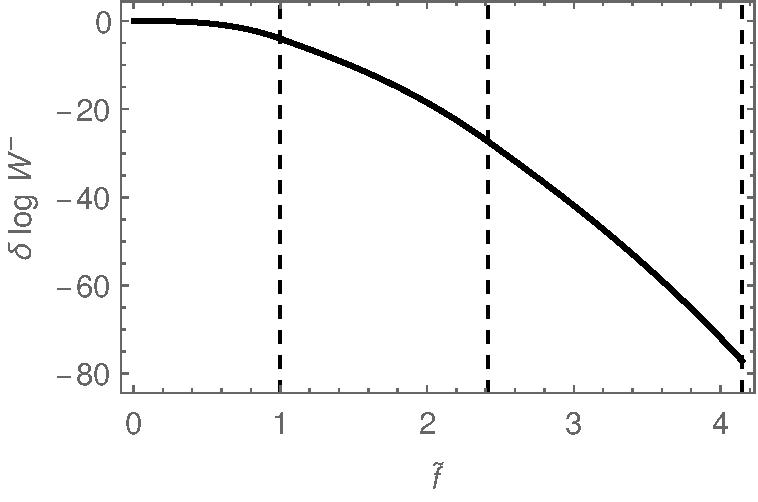
\includegraphics[width=0.49\textwidth]{Images/AntisymBlack.pdf} 
%   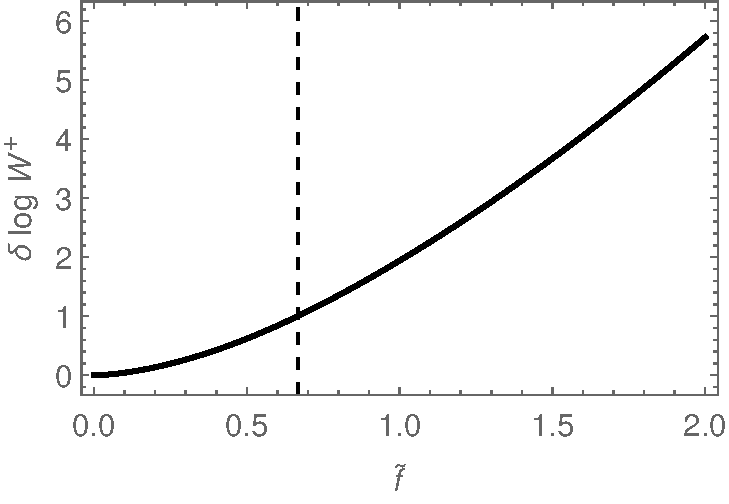
\includegraphics[width=0.49\textwidth]{Images/SymBlack.pdf} 
% \end{center}
% \caption{\label{fig:plotsCorrection} Strong coupling correction for the (rescaled) log of Wilson loops in 
% antisymmetric representation (left) with the critical points at $\{1, 1+\sqrt{2}, 1+\sqrt{2}+\sqrt{3},\ldots\}$,
% and in symmetric representation (right) with the critical point at $2/3$.}
% \end{figure}

\begin{figure}[t]
\begin{center}
 \centerline{ 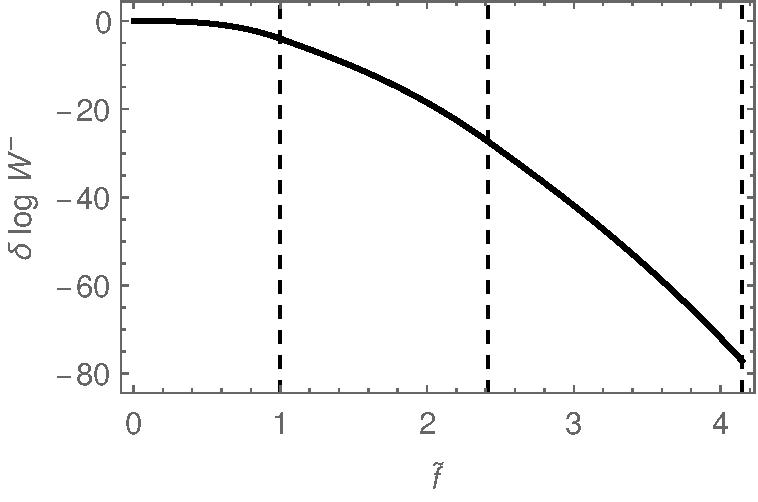
\includegraphics[width=0.8\textwidth]{Images/AntisymBlack.pdf} }
 \centerline{ 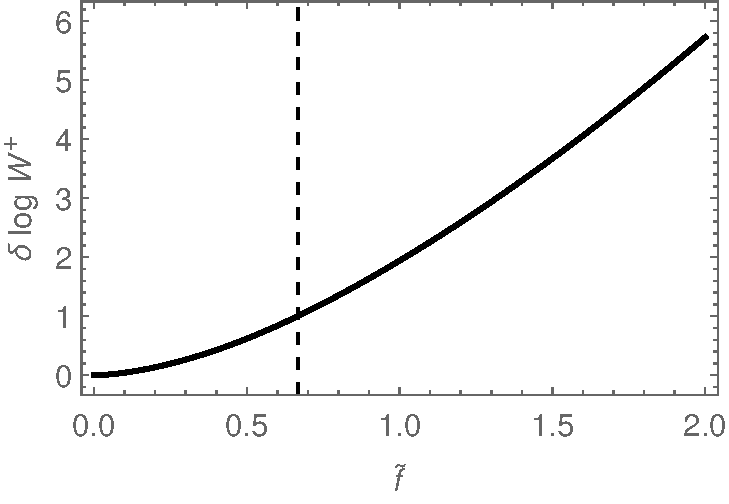
\includegraphics[width=0.8\textwidth]{Images/SymBlack.pdf} }
\end{center}
\caption{\label{fig:plotsCorrection} Strong coupling correction for (rescaled) log of Wilson loops in 
antisymmetric representation (up) with the critical points at $\{1, 1+\sqrt{2}, 1+\sqrt{2}+\sqrt{3},\ldots\}$,
and in symmetric representation (down) with the critical point at $2/3$.}
\end{figure}

